% Energy Quest · Student Sheet · MYP 1 Sciences · Al-Hayat International School
% XeLaTeX twice. Question numbers match the board pages (Q1.1 … Q6.1).
\documentclass[12pt,a4paper]{article}
\usepackage{hisstyle}
\renewcommand{\doctitle}{Energy Quest · Student Sheet}
\begin{document}
\thispagestyle{first}
\titleblock{Energy Quest}{Student sheet · Kinetic \& potential energy · Transformations · Energy resources}
\namerow

\begin{hook}[Statement of inquiry.]
Energy is never lost: it changes from one form to another, and the energy sources we choose change the world we live in.
\end{hook}
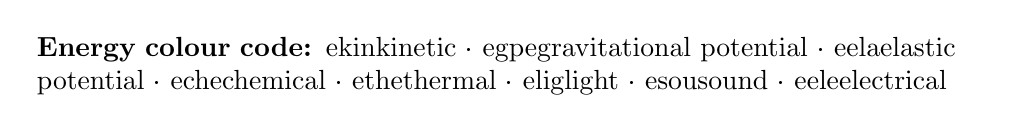
\begin{tikzpicture}\node[font=\normalsize,text width=\linewidth,align=left]{
\textbf{Energy colour code:} \e{ekin}{kinetic} · \e{egpe}{gravitational potential} · \e{eela}{elastic potential} · \e{eche}{chemical} · \e{ethe}{thermal} · \e{elig}{light} · \e{esou}{sound} · \e{eele}{electrical}};\end{tikzpicture}

% ===================== STATION 1 =====================
\station{ekin}{Station 1}{Energy is everywhere}
\crit{A}\ Energy is what makes things \textbf{happen}: move, heat up, light up, make sound, grow.

\Q{Q1.1 Gut feeling.} The power just cut. List three things in your home that need energy, and where each one gets it.
\lines{2}
\begin{teaser}[Q1.2 Brain teaser:]
Which two stores are called \emph{potential} energy? Why that name?
\lines{2}
\end{teaser}
\Q{Q1.3} Write the main energy store for each object: \textbf{K} kinetic, \textbf{G} gravitational potential, \textbf{E} elastic potential, \textbf{C} chemical.\par\vspace{2pt}
\begin{tabular}{@{}l c @{\hspace{8mm}} l c @{\hspace{8mm}} l c@{}}
rolling football & \bx[0.8cm] & apple hanging on a tree & \bx[0.8cm] & stretched rubber band & \bx[0.8cm]\\
wind blowing & \bx[0.8cm] & water behind a dam & \bx[0.8cm] & squashed spring & \bx[0.8cm]\\
running dog & \bx[0.8cm] & book on a high shelf & \bx[0.8cm] & pulled-back bow & \bx[0.8cm]\\
bread & \bx[0.8cm] & phone battery & \bx[0.8cm] & petrol & \bx[0.8cm]\\
\end{tabular}

\begin{multicols}{2}
\begin{teaser}[Q1.4 Brain teaser:]
Does a book sitting still on a high shelf have energy? How could you prove it?
\lines{2}
\end{teaser}
\columnbreak
\begin{real}[Q1.5 Real world:]
Your phone is on 10\%. Which store is in the battery? Name 3 things it turns into when you play a game.
\lines{2}
\end{real}
\end{multicols}

% ===================== STATION 2 =====================
\station{egpe}{Station 2}{Kinetic \& potential}
\crit{A}\ \crit{C}\ \e{ekin}{Kinetic}: faster or heavier → more. \e{egpe}{Gravitational potential}: higher or heavier → more.

\begin{minipage}[c]{0.47\linewidth}
\begin{tikzpicture}[scale=0.82]
  \draw[line width=2pt,muted,fill=panel] plot[domain=-3.6:3.6,samples=60] (\x,{0.27*\x*\x}) -- (3.6,-0.2) -- (-3.6,-0.2) -- cycle;
  \fill[egpe] (-3.3,{0.27*3.3*3.3}) circle (0.17) node[left=3pt,font=\bfseries] {A};
  \fill[egpe] (-1.9,{0.27*1.9*1.9}) circle (0.17) node[left=3pt,font=\bfseries] {B};
  \fill[ekin] (0,0) circle (0.17) node[below=4pt,font=\bfseries] {C};
  \fill[egpe] (2.6,{0.27*2.6*2.6}) circle (0.17) node[right=3pt,font=\bfseries] {D};
\end{tikzpicture}
\end{minipage}\hfill
\begin{minipage}[c]{0.5\linewidth}
\Q{Q2.1} A skater starts at A. Write the letter where:\par
most \e{ekin}{kinetic} energy: \bx[0.8cm]\par\vspace{3pt}
most \e{egpe}{gravitational potential}: \bx[0.8cm]\par\vspace{3pt}
the skater is fastest: \bx[0.8cm]
\end{minipage}

\Q{Q2.2} With \textbf{no friction}, what happens to the TOTAL energy? What does this tell you?
\lines{2}
\Q{Q2.3} With \textbf{a lot of friction}, why does the skater go less high each time? Where does the energy go?
\lines{2}
\begin{teaser}[Q2.4 Brain teaser:]
A 30 kg and a 70 kg skater start at the same height (no friction). Who is faster at the bottom? Who has more energy?
\lines{2}
\end{teaser}
\Q{Q2.5} \textbf{Bounce lab} (basketball). Record the heights, then describe the pattern.\par\vspace{2pt}
\begin{center}
\begin{tabular}{|l|C{2.2cm}|C{2.2cm}|C{2.2cm}|C{2.2cm}|C{2.2cm}|}
\hline\rowcolor{panel}\textbf{Height (m)} & \textbf{Drop} & \textbf{Bounce 1} & \textbf{Bounce 2} & \textbf{Bounce 3} & \textbf{Bounce 4}\\\hline
Basketball & & & & & \\\hline
\end{tabular}
\end{center}
Pattern: \lines{1}
\begin{teaser}[Q2.6 Brain teaser:]
Why can a dropped ball never bounce higher than where it started? Where does the "missing" energy go?
\lines{2}
\end{teaser}
\begin{multicols}{2}
\begin{real}[Q2.7 Real world:]
The Jounieh–Harissa cable car climbs. Which store increases? Where does it come from?
\lines{2}
\end{real}
\columnbreak
\begin{real}[Q2.8 Real world:]
Why is the first hill of a roller coaster always the tallest?
\lines{2}
\end{real}
\end{multicols}

% ===================== STATION 3 =====================
\station{eela}{Station 3}{Energy transformations}
\crit{A}\ Energy is \textbf{never created or destroyed}: it only changes form. Energy in = energy out.

\Q{Q3.1} The chain-reaction machine: write each energy change and its change-maker.\par\vspace{2pt}
\begin{tabular}{|C{0.8cm}|p{3.0cm}|p{6.6cm}|p{4.6cm}|}
\hline\rowcolor{panel}\textbf{Step} & \textbf{Object} & \textbf{Energy change (from → to)} & \textbf{Change-maker}\\\hline
1 & spring & & \\\hline
2 & ball on ramp & & \\\hline
3 & dominoes & & \\\hline
4 & bell & & \\\hline
5 & battery + lamp & & \\\hline
\end{tabular}

\Q{Q3.2} Write the change-maker: \textbf{F} force, \textbf{H} heating, \textbf{E} electric current, \textbf{R} chemical reaction, \textbf{L} light.\par\vspace{2pt}
\begin{tabular}{@{}l c @{\hspace{6mm}} l c@{}}
an apple falls from a tree & \bx[0.8cm] & a toaster's wires glow & \bx[0.8cm]\\
rubbing your hands to warm them & \bx[0.8cm] & a fan starts to spin & \bx[0.8cm]\\
kicking a football & \bx[0.8cm] & wood burning in a campfire & \bx[0.8cm]\\
an ice cube melts in your hand & \bx[0.8cm] & your body digesting lunch & \bx[0.8cm]\\
a pan warms on a hot stove & \bx[0.8cm] & a solar panel charges a lamp & \bx[0.8cm]\\
\end{tabular}

\Q{Q3.3} Device detective: energy \textbf{in} and main \textbf{useful} energy out.\par\vspace{2pt}
\begin{tabular}{|p{4.6cm}|p{5.6cm}|p{5.6cm}|}
\hline\rowcolor{panel}\textbf{Device} & \textbf{Energy in} & \textbf{Useful energy out}\\\hline
toaster & & \\\hline torch (battery) & & \\\hline wind turbine & & \\\hline loudspeaker & & \\\hline
bow and arrow & & \\\hline car engine & & \\\hline solar panel & & \\\hline water falling at a dam & & \\\hline
\end{tabular}

\Q{Q3.4} Bulb battle: which bulb wastes more energy? Why do families running on solar batteries choose LEDs?
\lines{2}
\Q{Q3.5} A kettle takes in 200 J. 150 J heats the water. Wasted energy = \blank[2cm] J.\quad Show working: \blank[5cm]
\begin{teaser}[Q3.6 Brain teaser:]
If energy is never destroyed, why do we keep paying for electricity and fuel?
\lines{2}
\end{teaser}
\Q{Q3.7} The neighbourhood diesel generator: complete the chain and name two wasted forms.\par\vspace{2pt}
\begin{tikzpicture}[x=1cm]
\node[ebox] (a) at (0,0) {diesel\\ \blank[2.2cm]}; \node[ebox] (b) at (4.3,0) {engine\\ \blank[2.2cm]}; \node[ebox] (c) at (8.6,0) {generator\\ \blank[2.2cm]}; \node[ebox] (d) at (12.9,0) {lamp\\ \blank[2.2cm]};
\draw[arr] (a) -- (b); \draw[arr] (b) -- (c); \draw[arr] (c) -- (d);
\node[anchor=west] at (-1.5,-1.25) {Wasted: \blank[3.6cm] and \blank[3.6cm]};
\end{tikzpicture}

% ===================== STATION 4 =====================
\station{eren}{Station 4}{Power the town}
\crit{A}\ \crit{D}\ \e{eren}{Renewable}: will not run out. \e{enon}{Non-renewable}: will run out (took millions of years to form).

\Q{Q4.1} Write \textbf{R} (renewable) or \textbf{N} (non-renewable).\par\vspace{2pt}
\begin{tabular}{@{}l c @{\hspace{6mm}} l c @{\hspace{6mm}} l c@{}}
sunlight & \bx[0.8cm] & coal & \bx[0.8cm] & heat from the Earth & \bx[0.8cm]\\
wind & \bx[0.8cm] & oil / diesel & \bx[0.8cm] & olive-pit fuel & \bx[0.8cm]\\
moving water & \bx[0.8cm] & natural gas & \bx[0.8cm] & uranium & \bx[0.8cm]\\
\end{tabular}
\begin{teaser}[Q4.2 Brain teaser:]
Where did the energy stored in fossil fuels originally come from?
\lines{1}
\end{teaser}
\Q{Q4.3} My team's town design.\par\vspace{2pt}
\begin{tabular}{|p{6.2cm}|C{2.6cm}|C{2.2cm}|C{2.2cm}|}
\hline\rowcolor{panel}\textbf{Sources we built} & \textbf{Lights on (\%)} & \textbf{CO\textsubscript{2}} & \textbf{Score}\\\hline
 & & & \\[6pt]\hline
\end{tabular}\par
With only solar farms, what happened at night? How could you fix it without fossil fuels?
\lines{2}
\Q{Q4.4} Why are fossil-fuel power plants still useful, even though they pollute?
\lines{2}
\Q{Q4.5} Solar panels and diesel generators in Lebanon.\par\vspace{2pt}
\begin{tabular}{|p{3.2cm}|p{6.4cm}|p{6.4cm}|}
\hline\rowcolor{panel} & \textbf{Advantages} & \textbf{Disadvantages}\\\hline
Solar panels & & \\[18pt]\hline
Diesel generator & & \\[18pt]\hline
\end{tabular}
\begin{multicols}{2}
\begin{real}[Q4.6 Real world:]
One way rooftop solar helps families, one way it helps the environment, and one problem it does not solve.
\lines{3}
\end{real}
\columnbreak
\begin{real}[Q4.7 Real world:]
Write the energy chain of the Qaraoun dam.
\lines{3}
\end{real}
\end{multicols}
\needspace{6\baselineskip}\Q{Q4.8 Debatable.} "Lebanon should get ALL of its electricity from renewable sources." My opinion, one reason for, one reason against:
\lines{3}

% ===================== STATION 5 =====================
\station{esou}{Station 5}{The lab: ramp racers}
\crit{B}\ \crit{C}\ Does the release height change how far a toy car rolls?

\Q{Q5.1} Research question: How does the \blank[4.6cm] affect the \blank[4.6cm]?

\Q{Q5.2} Hypothesis: If \blank[4.5cm], then \blank[5cm] because
\lines{2}
\Q{Q5.3} Variables.\par\vspace{2pt}
\begin{tabular}{|p{4.4cm}|p{11.6cm}|}
\hline
Independent variable (I change) & \\\hline
Dependent variable (I measure) & \\\hline
Controlled variables (4) & 1. \hspace{5cm} 2.\\
 & 3. \hspace{5cm} 4.\\\hline
\end{tabular}

\Q{Q5.4} Method (numbered steps). Include how you change the height, how you measure, and how many repeats.
\lines{5}

\Q{Q5.5} Results (\textbf{tiled corridor}). Calculate each average: (trial 1 + trial 2 + trial 3) ÷ 3.\par\vspace{2pt}
\begin{center}
\begin{tabular}{|C{3.6cm}|C{2.5cm}|C{2.5cm}|C{2.5cm}|C{3.0cm}|}
\hline\rowcolor{panel}\textbf{Release height (cm)} & \textbf{Trial 1 (cm)} & \textbf{Trial 2 (cm)} & \textbf{Trial 3 (cm)} & \textbf{Average (cm)}\\\hline
10 & & & & \\\hline 20 & & & & \\\hline 30 & & & & \\\hline 40 & & & & \\\hline 50 & & & & \\\hline
\end{tabular}
\end{center}
\noindent\begin{minipage}{\linewidth}Plot the averages (choose a scale for each axis) and draw a best-fit line.
\begin{center}\gridgraph{14cm}{8.2cm}{Release height (cm)}{Average distance rolled (cm)}\end{center}\end{minipage}
\Q{Q5.6} Describe the trend. Use numbers from your data.
\lines{2}
\Q{Q5.7} Was your hypothesis supported? Explain using energy.
\lines{3}
\Q{Q5.8} Anomaly: which result does not fit? Possible cause? What should you do?
\lines{2}
\Q{Q5.9} Evaluation: two problems with the method and an improvement for each.
\lines{4}
\begin{teaser}[Q5.10 Extension:]
On carpet the results are different. Describe the difference and explain it.
\lines{2}
\end{teaser}

% ===================== STATION 6 =====================
\station{hisblue}{Station 6}{The challenge: GRASPS planner}
\crit{D}\ Plan your poster or presentation: an energy plan for our school.

\begin{tabular}{|p{3.2cm}|p{12.8cm}|}
\hline\rowcolor{panel}\multicolumn{2}{|l|}{\textbf{1 · Energy transformation diagrams} (show useful and wasted energy)}\\\hline
Diesel generator & \\[26pt]\hline
My new system & \\[26pt]\hline
\rowcolor{panel}\multicolumn{2}{|l|}{\textbf{2 · My energy sources} (renewable or non-renewable? 2 advantages, 2 disadvantages each)}\\\hline
Source 1: & \\[26pt]\hline
Source 2: & \\[26pt]\hline
\rowcolor{panel}\multicolumn{2}{|l|}{\textbf{3 · One way to waste less energy}}\\\hline
 & \\[14pt]\hline
\rowcolor{panel}\multicolumn{2}{|l|}{\textbf{4 · Effects of my plan}}\\\hline
People & \\[14pt]\hline Money & \\[14pt]\hline Environment & \\[14pt]\hline
\rowcolor{panel}\multicolumn{2}{|l|}{\textbf{5 · My sources} (title, author or organization, date, link)}\\\hline
1 & \\[8pt]\hline 2 & \\[8pt]\hline
\end{tabular}

\Q{Q6.1 Exit ticket.} \textbf{3} energy transformations I saw today in real life:
\lines{2}
\textbf{2} things I will tell my family about saving energy:
\lines{2}
\textbf{1} question I still have: \blank[11cm]
\end{document}
